\subsubsection{Application of the Confidence Connected filter on the Brain Web Data}
This section shows some results obtained by applying the Confidence Connected filter on the BrainWeb database. The filter was applied on a 181 $\times$ 217 $\times$ 181 crosssection of the {\it brainweb165a10f17} dataset. The data is a MR T1 acquisition, with an intensity non-uniformity of 20\% and a slice thickness 1mm. The dataset may be obtained from
\code{http://www.bic.mni.mcgill.ca/brainweb/} or
\code{https://data.kitware.com/\#folder/5882712d8d777f4f3f3072df}

The previous code was used in this example replacing the image dimension by 3.
Gradient Anistropic diffusion was applied to smooth the image. The filter used 2 iterations, a time step of 0.05 and a conductance value of 3. The smoothed volume was then segmented using the Confidence Connected approach. Five seed points were used at coordinate locations (118,85,92), (63,87,94), (63,157,90), (111,188,90), (111,50,88). The ConfidenceConnnected filter used the parameters, a neighborhood radius of 2, 5 iterations and an $f$ of 2.5 (the same as in the previous example). The results were then rendered using VolView.

Figure \ref{fig:3DregionGrowingScreenshot1} shows the rendered volume. Figure \ref{fig:SlicesBrainWeb} shows an axial, saggital and a coronal slice of the volume.

\begin{figure}
\centering
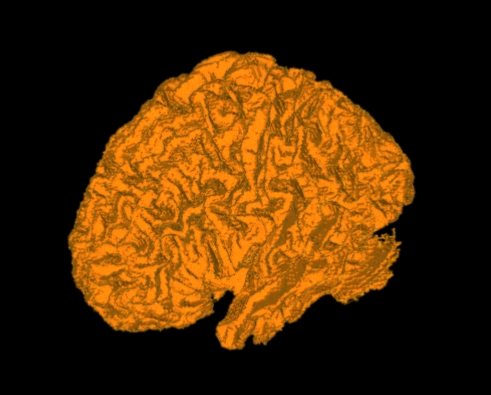
\includegraphics[width=0.6\textwidth]{3DregionGrowingScreenshot1.eps}
\itkcaption[Whitematter Confidence Connected segmentation.]{White matter segmented using Confidence Connected region growing.}
\label{fig:3DregionGrowingScreenshot1}
\end{figure}

\begin{figure}
\centering

\includegraphics[width=\textwidth]{SlicesBrainWebConfidenceConnected.eps}
\itkcaption[Axial, sagittal, and coronal slice of Confidence Connected segmentation.]{Axial, sagittal and coronal slice segmented using Confidence Connected region growing.}
\label{fig:SlicesBrainWeb}
\end{figure}
